\subsection{Maps \& Templates}

The templates were given at the very beginning of the file, at Table \ref{templates}. Beneath follows some more in depth analysis on each map and template specifically for SR templates.
\\
\\
The recipe behind the Vanilla templates is straight forward. In the MTL there are 19 in this category, plus three more I'm including here due to how similar the design is (Guiroma, BFME, Tarabonia's Choice), as seen first in Tables \ref{table:sr_opening_sorted}, \ref{table:sr_bonus_sorted} and \ref{table:sr_ratios_sorted}.

%--------------- Straight-Round opening economy (sorted by Arm/InitTerr, then Base inc) ---------------
\scriptsize
\begin{longtable}{|l|c|c|c|c|c|c|c|c|}
\hline
\rowcolor{Baby_Blue}
Template & Move & Init & Arm/\newline Init & Neutr & Neutr in & Wastelands & Wasteland & Base \\ 
\rowcolor{Baby_Blue}
(Name)   & order & terr & terr           & Size & Dist & (\#)  & Size & Income \\ \hline\hline
\endfirsthead
\hline
\rowcolor{Baby_Blue}
Template & Move & Init & Arm/\newline Init & Neutr & Neutr in Dist & Wasts & Waste sz & Base inc \\ \hline\hline
\endhead
% ---- Arm/Init = 5 ----------------------------------------------------------
Strategic Greece            & random & 5 & 5 & 2 & 3 & 10 & 6 & 5 \\ \hline
Guiroma                      & random & 4 & 5 & 2 & 4 & 15 & 3 & 5 \\ \hline \hline \hline
% ---- Arm/Init = 4  |  Base inc = 5 ----------------------------------------
Basileia                     & random & 3 & 4 & 2 & 4 & 10 & 3 & 5 \\ \hline
Battle for Middle Earth      & random & 4 & 4 & 2 & 4 & 10 &10 & 5 \\ \hline
Battle Islands V            & cycle  & 3 & 4 & 2 & 4 & 5  &15 & 5 \\ \hline
Black Sea                    & random & 4 & 4 & 2 & 2 & 6  &10 & 5 \\ \hline
Malvia                       & cycle  & 4 & 4 & 2 & 3 & 6  &10 & 5 \\ \hline
Post-melt Antarctica         & cycle  & 3 & 4 & 2 & 0 & 7  & 4 & 5 \\ \hline
Strat MME                    & cycle  & 3 & 4 & 2 & 4 & 7  &10 & 5 \\ \hline
Volcano Island               & cycle  & 4 & 4 & 2 & 4 & 5  &10 & 5 \\ \hline
World of Warhammer           & random & 4 & 4 & 2 & 4 & 8  &10 & 5 \\ \hline \hline \hline
% ---- Arm/Init = 4  |  Base inc = 4 ----------------------------------------
Greater Middle East III      & random & 4 & 4 & 2 & 4 & 5  &10 & 4 \\ \hline
Laketown                     & random & 4 & 4 & 2 & 3 &10 & 3 & 4 \\ \hline
Saudi Arabia                 & cycle  & 4 & 4 & 2 & 3 & 4 & 5 & 4 \\ \hline
Tarabonia's Choice           & cycle  & 3 & 4 & 2 & 4 & 4 &10 & 4 \\ \hline
Treasure Map                 & cycle  & 4 & 4 & 2 & 4 & 6 & 7 & 4 \\ \hline \hline \hline
% ---- Arm/Init = 3  |  Base inc = 5 ----------------------------------------
Unicorn Island               & cycle  & 5 & 3 & 2 & 4 & 3 &10 & 5 \\ \hline
% ---- Arm/Init = 3  |  Base inc = 4 ----------------------------------------
Discovery                    & cycle  & 4 & 3 & 6 & 2 & 80 & 2 & 4 \\ \hline
Hannibal at the Gates        & random & 5 & 3 & 2 & 2 & 12 & 3 & 4 \\ \hline
% ---- Arm/Init = 3  |  Base inc = 3 ----------------------------------------
Australia                    & cycle  & 5 & 3 & 2 & 3 & 60 & 2 & 3 \\ \hline
Numenor                      & cycle  & 5 & 3 & 2 & 4 & 20 & 3 & 3 \\ \hline \hline \hline
% ---- Arm/Init = 2 ----------------------------------------------------------
Slow Burn                    & cycle  & 3 & 2 & 2 & 3 & 8  &12 & 3 \\ \hline
\caption{Straight-Round templates sorted by (Armies per Initial Territory) and then by Base Income.}
\label{table:sr_opening_sorted}
\end{longtable}
\normalsize

%--------------- Straight-Round bonus geometry (sorted by Arm/Init, then Base inc) ---------------
\scriptsize
\begin{longtable}{|l|c|c|c|c|c|c|c|c|}
\hline
\rowcolor{Baby_Blue}
Template & Arm/\newline Init & Base & Tot & Distr & Bonuses & Over- & Effi- & Bonus– \\ 
\rowcolor{Baby_Blue}
(Name)   & Terr & inc & Terr & mode & > 0 & lap & ciency & count \\ \hline\hline
\endfirsthead
\hline
\rowcolor{Baby_Blue}
Template & Arm/\newline Init & Base & Tot & Distr & Bonuses & Over- & Effi- & Bonus– \\ \hline\hline
\endhead
% ---- Arm/Init = 5 ----------------------------------------------------------
Strategic Greece          & 5 & 5 & 103 & RWD & 24 & 0 & n-1 & 24 \\ \hline
Guiroma                   & 5 & 5 & 106 & RWD & 26 & 0 & n-1 & 23 \\ \hline\hline\hline
% ---- Arm/Init = 4 | Base inc = 5 ------------------------------------------
Basileia                  & 4 & 5 &  80 & RWD & 22 & 0 & n-1 & 22 \\ \hline
Battle for Middle Earth   & 4 & 5 & 167 & RWD & 32 & 0 & n-1 & 14 \\ \hline
Battle Islands V          & 4 & 5 & 134 & RWD & 24 & 0 & n-1 & 18 \\ \hline
Black Sea                 & 4 & 5 & 114 & RWD & 27 & 0 & n-1 & 27 \\ \hline
Malvia                    & 4 & 5 & 129 & RWD & 28 & 0 & n-1 & 25 \\ \hline
Post-melt Antarctica      & 4 & 5 &  96 & RWD & 18 & 0 & n-2 & 18 \\ \hline
Strat MME                 & 4 & 5 & 129 & RWD & 23 & 0 & n-1 & 17 \\ \hline
Volcano Island            & 4 & 5 & 123 & RWD & 23 & 1 & n-1 & 22 \\ \hline
World of Warhammer        & 4 & 5 & 137 & RWD & 25 & 0 & n-1 & 19 \\ \hline\hline\hline
% ---- Arm/Init = 4 | Base inc = 4 ------------------------------------------
Greater Middle East III   & 4 & 4 & 140 & RWD & 30 & 0 & n-1 & 17 \\ \hline
Laketown                  & 4 & 4 & 109 & RWD & 23 & 0 & n-1 & 23 \\ \hline
Saudi Arabia              & 4 & 4 &  81 & RWD & 18 & 0 & n-1 & 14 \\ \hline
Tarabonia's Choice        & 4 & 4 & 132 & RWD & 28 & 0 & n-2 & 28 \\ \hline
Treasure Map              & 4 & 4 & 137 & RWD & 27 & 0 & n-1 & 19 \\ \hline\hline\hline
% ---- Arm/Init = 3 | Base inc = 5 ------------------------------------------
Unicorn Island            & 3 & 5 & 153 & RWD & 27 & 0 & n-1 & 12 \\ \hline
% ---- Arm/Init = 3 | Base inc = 4 ------------------------------------------
Discovery                 & 3 & 4 & 128 & RCD & 34 & 0 & n-1 & 34 \\ \hline
Hannibal at the Gates     & 3 & 4 &  83 & RWD & 25 & 0 & n-1 & 25 \\ \hline
% ---- Arm/Init = 3 | Base inc = 3 ------------------------------------------
Australia                 & 3 & 3 & 111 & RWD & 49 & 13 & n   & 23 \\ \hline
Numenor                   & 3 & 3 & 159 & RWD & 49 & 6 & n-1 & 18 \\ \hline\hline\hline
% ---- Arm/Init = 2 ----------------------------------------------------------
Slow Burn                 & 2 & 3 & 134 & RWD & 24 & 0 & n-1 & 24 \\ \hline
\caption{Straight-Round templates sorted first by Armies-per-Initial-Territory, then by Base income.}
\label{table:sr_bonus_sorted}
\end{longtable}
\normalsize

%--------------- Straight-Round density & wasteland ratios (sorted by Arm/Init, then Base inc) ---------------
\scriptsize
\begin{longtable}{|l|c|c|c|c|c|c|c|c|}
\hline
\rowcolor{Baby_Blue}
Template & Init & Arm/\newline Init & Base & Init/ & Init/ & Init/ & WL/\newline Terr & WL/\newline Bonus \\ 
\rowcolor{Baby_Blue}
(Name)   & Terr & Terr             & inc  & Terr  & Bonus & Eff.\ Bonus & (RWD) & (RWD) \\ \hline\hline
\endfirsthead
\hline
\rowcolor{Baby_Blue}
Template & Init & Arm/\newline Init & Base & Init/ & Init/ & Init/ & WL/\newline Terr & WL/\newline Bonus \\ \hline\hline
\endhead
% ---- Arm/Init = 5 ----------------------------------------------------------
Strategic Greece          & 5 & 5 & 5 & 4.85 & 20.83 & 20.83 & 9.71 & 41.67 \\ \hline
Guiroma                   & 4 & 5 & 5 & 3.77 & 15.38 & 17.39 & 14.15 & 57.69 \\ \hline\hline\hline
% ---- Arm/Init = 4 | Base inc = 5 ------------------------------------------
Basileia                  & 3 & 4 & 5 & 3.75 & 13.64 & 13.64 & 12.50 & 45.45 \\ \hline
Battle for Middle Earth   & 4 & 4 & 5 & 2.40 & 12.50 & 28.57 & 5.99 & 31.25 \\ \hline
Battle Islands V          & 3 & 4 & 5 & 2.24 & 12.50 & 16.67 & 3.73 & 20.83 \\ \hline
Black Sea                 & 4 & 4 & 5 & 3.51 & 14.81 & 14.81 & 5.26 & 22.22 \\ \hline
Malvia                    & 4 & 4 & 5 & 3.10 & 14.29 & 16.00 & 4.65 & 21.43 \\ \hline
Post-melt Antarctica      & 3 & 4 & 5 & 3.13 & 16.67 & 16.67 & 7.29 & 38.89 \\ \hline
Strat MME                 & 3 & 4 & 5 & 2.33 & 13.04 & 17.65 & 5.43 & 30.43 \\ \hline
Volcano Island            & 4 & 4 & 5 & 3.25 & 17.39 & 18.18 & 4.07 & 21.74 \\ \hline
World of Warhammer        & 4 & 4 & 5 & 2.92 & 16.00 & 21.05 & 5.84 & 32.00 \\ \hline\hline\hline
% ---- Arm/Init = 4 | Base inc = 4 ------------------------------------------
Greater Middle East III   & 4 & 4 & 4 & 2.86 & 13.33 & 23.53 & 3.57 & 16.67 \\ \hline
Laketown                  & 4 & 4 & 4 & 3.67 & 17.39 & 17.39 & 9.17 & 43.48 \\ \hline
Saudi Arabia              & 4 & 4 & 4 & 4.94 & 22.22 & 28.57 & 4.94 & 22.22 \\ \hline
Tarabonia's Choice        & 3 & 4 & 4 & 2.27 & 10.71 & 10.71 & 3.03 & 14.29 \\ \hline
Treasure Map              & 4 & 4 & 4 & 2.92 & 14.81 & 21.05 & 4.38 & 22.22 \\ \hline\hline\hline
% ---- Arm/Init = 3 | Base inc = 5 ------------------------------------------
Unicorn Island            & 5 & 3 & 5 & 3.27 & 18.52 & 41.67 & 1.96 & 11.11 \\ \hline
% ---- Arm/Init = 3 | Base inc = 4 ------------------------------------------
Discovery                 & 4 & 3 & 4 & 3.13 & 11.76 & 11.76 & --   & --   \\ \hline
Hannibal at the Gates     & 5 & 3 & 4 & 6.02 & 20.00 & 20.00 & 14.46 & 48.00 \\ \hline
% ---- Arm/Init = 3 | Base inc = 3 ------------------------------------------
Australia                 & 5 & 3 & 3 & 4.50 & 10.20 & 21.74 & 54.05 & 122.45 \\ \hline
Numenor                   & 5 & 3 & 3 & 3.14 & 10.20 & 27.78 & 12.58 & 40.82 \\ \hline\hline\hline
% ---- Arm/Init = 2 ----------------------------------------------------------
Slow Burn                 & 3 & 2 & 3 & 2.24 & 12.50 & 12.50 & 5.97 & 33.33 \\ \hline
\caption{Straight-Round templates sorted by Armies-per-Initial-Territory, then by Base income; showing density and wasteland ratios.}
\label{table:sr_ratios_sorted}
\end{longtable}
\normalsize

Takeaways:
\begin{itemize}
    \item All 22 templates take place in small maps of the size between 81-167 territories. Generally speaking, the game is more brawly in smaller maps, and more expansion heavy in larger maps. However, you can see in \ref{table:sr_bonus_sorted} the very last column which counts the number of efficient bonuses in that template. For example, BFME takes place in a map of 167 territories with 32 bonuses, but 14/32 are actually decent. The ratio of number of initial territories divided by number of efficient bonuses is given on \ref{table:sr_ratios_sorted} column "Init/Bonus". The higher the value, the brawlier the template, the more important really fast income is. Of course, each template has something unique to it, that changes gameplay.
    \item There's four major parameters that control the gameplay (with some extra that can influence things like the rf card).
    \begin{enumerate}
        \item Wastelands (number and size)
        \begin{itemize}
            \item Wastelands nullify some bonuses in an attempt to a) introduce variety in each template from game to game and b) limit the number of ideas in picksets that are possible. It is directly correlated with the strategicness of a template. A distribution in MME with 0 wastelands allows for way too many possible picksets that you simply cannot account for with 1 idea, introducing luck. However, it's not enough by itself, there's always a pickset to counter another pickset. Luck is an inherent part of SR vanilla templates, even at small amounts.
            \item You'll find that some templates have smaller size wastelands, introducing some difficulty in completing a bonus but not prohibing capture, in templates like Guiroma, Basileia and even Strategic Greece. While in other templates, wastelands are so big they define the map.
            \item In Table \ref{table:sr_ratios_sorted}, the column WL/Bonus (RWD) gives the number of wastelands, times 100, divided by the number of efficient bonuses in the template, to give an estimator of the amount of wastelands compared to the amount of bonuses in play. You'll find generally that templates with higher ratio, have more forced picks, while templates with lower ratio allow a lot of different ideas during picks. 
            \item Regardless, you can see a sweet spot at 20-35 \% ratio. Higher, is often accompanied with low size of wastelands (Guiroma, Basileia, Laketown, Hannibal at the Gates, Numenor) or in the case of Strategic Greece, a very brawly game. Lower than that is only observed in GME III, Tarabonia's Choice and Unicorn Island, with all 3 having a very distinct playstyle of trying your best to flank your opponent at the other side of the board. 
        \end{itemize}
        \item Differentiating bonuses in efficiency depending on the map connections
        \begin{itemize}
            \item Reverse the argument. Some of the templates in this list where every bonus is equally efficient are Strategic Greece and Slow Burn. Both of these come with more wastelands than the average template.
            \item Another way to limit the number of possible picksets is through changing the values of some bonuses to force choices in picks. Templates like Australia, BFME, World of Warhammer, come with compartmentalized areas of the map which are far superior and change the way you approach picks, as well as gameplay.
        \end{itemize}
        \item Armies per Initial Territory with Income
        \begin{itemize}
            \item High Income templates / High Armies per Initial Territory  -> Expansion is easier -> Earlier contact \& fights. 
            \item Low Income / Low Armies per Initial Territory  -> Expansion slower -> Contact later
            \item High No of Initial Territories -> More coverage of the map -> Earlier Fights
            \item Low No of Initial Territories -> Less coverage of the map -> Contact later
        \end{itemize}
        \item Neutrals and Neutrals in Distribution
        \begin{itemize}
            \item All templates come with neutrals of 2 as of this moment. (Neutrals of 6 in Discovery has to do with RCD distribution mode). The size 2 allows fast and efficient expansion (-1 attacker at 60:70 kill rates). Though there is room for experimentation with different numbers.
            \item Neutrals in distribution comes as another parameter that can affect gameplay. For example, in templates where that number is different than 2, seeing a bonus with a 4 army neutral for example inside, means your opponent didn't spawn there, providing you with some relative safety after picks. 
            \item Neutrals in distribution of 2/3 allow faster and easier expansion. Size of 4 exists as an obstacle for expanding into different bonuses to slow down the game.
        \end{itemize}
    \end{enumerate}
\end{itemize}

\subsubsection{Efficient Bonuses}

Above, I referred to bonuses as n-1 or n-2, given:
\begin{itemize}
    \item n = territories in the bonus
    \item (n-1) or (n-2) or any similar value for the income the bonus gives back upon capturing
\end{itemize}

\begin{itemize}
    \item At (n) templates (where x number of territories give x number income back, like Australia), the static return of I/T is 1. Every bonus, tiny or huge, pays the same. So, if you have immediate contact to force plays, you pick smaller bonuses, 1:1 or 2:2. If not, 3:3 or bigger bonuses are viable.
    \item At (n-1) templates, the static return is between 0.75-0.86. 
    \begin{enumerate}
        \item 4 terr for 3 income is 0.75.
        \item 5 terr for 4 income is 0.8.
        \item 6 terr for 5 income is 0.83.
    \end{enumerate}
    As a result, always keep in mind that bigger bonuses slightly more efficient. You can imagine this by comparing two different positions in Strat MME, where player A has 2x +3 bonuses and a +4 bonus (total of 13 territories for 10 income) while player B has 2x +5 bonuses and a 3rd that doesn't matter - not completed yet (12 territories for 10 income). However, going for bigger bonuses comes with a cost that they are slower. Small bonuses finish faster and pay-out faster. Big bonuses are more efficient but take time. 
    \item At (n-2) templates (namely Antarctica and Tarabonia's Choice), the static return is between 0.62-0.71. Bigger bonuses are a lot more efficient than smaller ones. A +4 bonus in Tarabonia comes at 6 territories. If you pick 2x +1 bonuses also for 6 territories, that's +2 income in return. 
\end{itemize}

\begin{wrapfigure}{r}{0.40\textwidth}
    \centering
    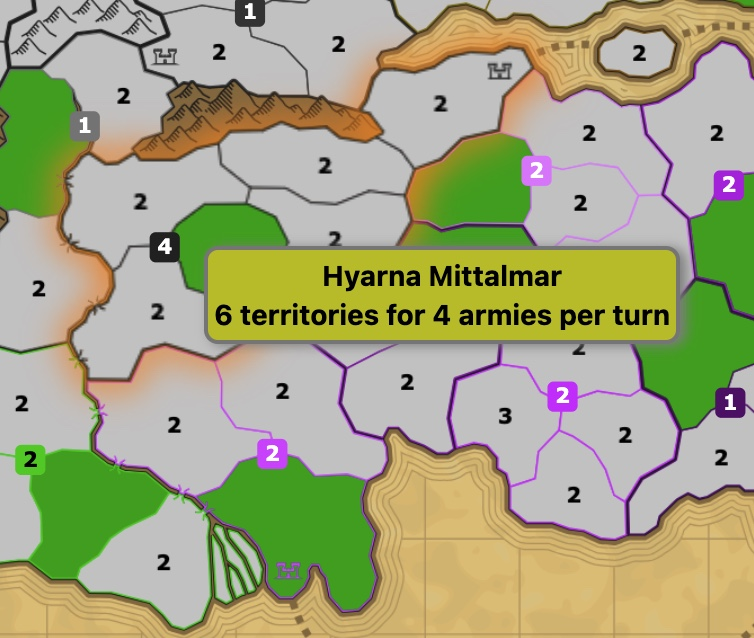
\includegraphics[width=0.40\textwidth]{Images/num4.jpg}
    \caption{6 Territories for +4 Income}
    \label{num4}
\end{wrapfigure}

So overall, efficiency isn't as simple as n-1, I just use that metric to categorize templates. The map size and the way the game plays out are equally if not more important, while some bonuses appear inefficient but aren't. Take a look at Figure \ref{num4} at the central +4 bonus in Numenor. 6 Territories for 4 Income. In theory (n-2) in a template with multiple (n-1) bonuses. However, consider Player A having 2x +2 bonuses of 3 territories each  (6 terr for 4 income) and Player B having 1x +4 bonus of 6 territories. Same outcome. What matters is a) the speed at which you can capture the bonus so you can invest that income faster elsewhere against your opponent and b) the safety of that bonus.
\\
\\
The templates above feature mostly bonuses that consist of 4-7 territories, with notable exceptions that push this to the 3-8 range. Smaller bonuses typically are too powerful (assuming they net income), while larger bonuses are too slow to finish. Only notable exceptions in this category are \href{https://www.warzone.com/MultiPlayer/Tournament?ID=52991}{Africa Ultima} and Laketown.
\\
\\
On a final note, don't take too granted that efficiency is always better. Ideally you should calculate how your pickset expands and plays out and how it plays out against other ideas. Picking in inefficient bonuses might also surprise your opponent. It's all relative. 
\\
\\
Outside of the above 22 templates, the MTL features 9 WR templates that follow the same principles of efficiency. Beyond that, there's a lot (20) of "case-specific" ones that feature ideas which define the template. The army cap templates are... about army cap and army management, similarly for the rest. 